\documentclass[11pt]{report}
\usepackage[abgabe]{protokoll}
\lstset{literate=
  {á}{{\'a}}1 {é}{{\'e}}1 {í}{{\'i}}1 {ó}{{\'o}}1 {ú}{{\'u}}1
  {Á}{{\'A}}1 {É}{{\'E}}1 {Í}{{\'I}}1 {Ó}{{\'O}}1 {Ú}{{\'U}}1
  {à}{{\`a}}1 {è}{{\`e}}1 {ì}{{\`i}}1 {ò}{{\`o}}1 {ù}{{\`u}}1
  {À}{{\`A}}1 {È}{{\'E}}1 {Ì}{{\`I}}1 {Ò}{{\`O}}1 {Ù}{{\`U}}1
  {ä}{{\"a}}1 {ë}{{\"e}}1 {ï}{{\"i}}1 {ö}{{\"o}}1 {ü}{{\"u}}1
  {Ä}{{\"A}}1 {Ë}{{\"E}}1 {Ï}{{\"I}}1 {Ö}{{\"O}}1 {Ü}{{\"U}}1
  {â}{{\^a}}1 {ê}{{\^e}}1 {î}{{\^i}}1 {ô}{{\^o}}1 {û}{{\^u}}1
  {Â}{{\^A}}1 {Ê}{{\^E}}1 {Î}{{\^I}}1 {Ô}{{\^O}}1 {Û}{{\^U}}1
  {œ}{{\oe}}1 {Œ}{{\OE}}1 {æ}{{\ae}}1 {Æ}{{\AE}}1 {ß}{{\ss}}1
  {ű}{{\H{u}}}1 {Ű}{{\H{U}}}1 {ő}{{\H{o}}}1 {Ő}{{\H{O}}}1  
  {ç}{{\c c}}1 {Ç}{{\c C}}1 {ø}{{\o}}1 {å}{{\r a}}1 {Å}{{\r A}}1
  {€}{{\EUR}}1 {£}{{\pounds}}1
}
\graphicspath{
  {pictures/}
}
\lstset{inputpath=source/}
\version{0.1$\alpha$}
\datum{\today}

%%
%% Titel, Autor und Betreuer
%%
\fachbereich{VII -- Elektrotechnik - Mechatronik - Optometrie --} 
\studiengang{Elektrotechnik - Schwerpunkt Elektronische Systeme}
\autor{Robby Kozok, Nic Frank Siebenborn, Pascal Kahlert}
\titel{DTMF-Detektor mit Goertzel-Algorithmus} 
\untertitel{Laborbericht}
\modul{Digitale Signalverarbeitung III}
\betreuerFeld{
  \begin{tabular}{lr}
    \multicolumn{2}{l}{\textbf{Lehrkraft}}\\
    Prof.~Dr.-Ing~Marcus~Purat & Beuth Hochschule für Technik\\
  \end{tabular}
}
%%
%% Abkürzungen
%%
\makenoidxglossaries

\newacronym{dtmf}{DTMF}{Dual-tone multi-frequency(Mehrfrequenzwahlverfahren)}





\begin{document}

\pagestyle{fancy}

%% Titelseite
\maketitle
\clearpage

%% Leerseite
\newpage

%\chapter*{Einleitung}

%% Einfügen des genutzten Aufgabenblattes. 
\clearpage
%% Seitenzahlen
\pagenumbering{roman}

%% Inhaltsverzeichnis
\tableofcontents

%% Abbildungsverzeichnis


%%Titelseite


\pagenumbering{arabic}


%%Kapitel
%%\chapter{Vorbereitung}

In folgender Tabelle sind die DTMF-Frequenzen sowie die normierten Kreisfrequenzen (Abtastfrequenz: 48kHz) zu sehen.\\

\begin{table}[H]
	
\centering
\begin{tabular}{l|l|l|l|l}
	Hz & 1209 & 1336 & 1477 & 1633 \\
	\begin{math}\Omega_n\end{math}  & 0,158257 & 0,174881 & 0,193338 & 0,213759\\
	\hline\hline 
	697 & & & & \\
	0,091237 & 1 & 2 & 3 & A \\
	\hline
	770 & & & & \\
	0,091237 & 4 & 5 & 6 & B \\
	\hline
	852 & & & & \\
	0,091237 & 7 & 8 & 9 & C \\
	\hline
	941 & & & & \\
	0,091237 & * & 0 & \# & D \\
	\hline
\end{tabular}\\
\end{table}

Die normierten Kreisfrequenzen errechnen sich nach folgender Formel:


\begin{equation}
  \Omega_n=\frac{2*\pi*f_{DTMF}}{48kHz}
\end{equation}

Nun soll mit folgenden Formeln die Ordnung der FFT bestimmt werden. 
\begin{equation}
  \Delta\Omega=\frac{2*\pi}{N}=2*\Pi*\frac{\Delta f}{f_T}
\end{equation}
Daraus folgt:
\begin{equation}
  N=\frac{f_T}{\Delta f}
\end{equation}
Die minimalste Frequenz \begin{math}\Delta f\end{math} befindet sich zwischen den DTMF-Frequenzen 697Hz und 770Hz.
Auch sollen laut Vorgabe 3 weitere St\"utzstellen verwendet werden, das macht insgesamt 4.
Daraus ergibt sich folgende Filterordnung.
\begin{equation}
  N=\frac{48kHz}{0,25*(770Hz-697Hz)}=2630,14
\end{equation}
Da wir eine Funktion aus der DSP Library verwenden bei der eine 2er Potenz von N ben\"otigt wird, m\"ussen wir ebenfalls eine Filterordnung mit 2er Potenz verwenden.
Dies macht eine Filterordnung von N=4096.
\chapter{Goerzel Algorithmus}\label{Goertzel}
In dem folgenden Kapitel wird die FFT ohne Fensterung untersucht. 
\section{Aufgabenstellung}\label{GoertzelAuf}
In dieser Aufgabe sollten der Goertzel und FFT Algorithmus verglichen werden. Im ersten Schritt sollten bei Ergebnisse für die 8 DTMF Frequenzen verglichen werden und im zweiten Schritt sollte betrachtet werden, welche der beiden Implementierungen einen höheren Rechenaufwand besitzt. 
\section{Durchführung}\label{GoertzelDur}
Bevor der Goertzel Algorithmus genutzt werden kann müssen seine Koeffizienten berechnet werden. Dies haben wir in einem Matlab Script (s. Code \autoref{code:GoertzelMatlab}) realisiert.\\
\lstinputlisting[caption={Berechnung der Goertzel Koeffizienten}, label={code:GoertzelMatlab}]{goertzelKoef.m}
In Zeile 1 bis 9 definieren wir die Positionen der DTMF Frequenzen. In den folgenden Zeilen berechnen wir für jeden Goertzel Filter die Koeffizienten.
Im Source Code ergibt sich dadurch ein Array wie in \autoref{code:goertzelKoef} dargestellt.
\begin{lstlisting}[caption={Array der Goertzel - Koeffizienten}, label={code:goertzelKoef}]
	fract16 coeff[16] = 
	{ 
	//ak	bk
	32634, 2962,
	32600, 3312,
	32563, 3662,
	32522, 4011,
	32360, 5156,
	32268, 5701, 
	32158, 6294,
	32026, 6934
	}
\end{lstlisting}
Im Vergleich zur Übung 4 musste nun anstatt des FFT Algorithmus der Goertzel Algorithmus genutzt werden.

Der Rechenaufwand wurde wie in Übung 2 bestimmt. 
\section{Auswertung}
Der Goertzel-Algorithmus lieferte uns nicht das erwartete Ergebnis. Wir erwarteten genau ein eindeutigs Maximum, dies erhielten wir aber nicht. Deswegen wird der DTMF Detektor im weiteren nicht mehr betrachtet.
\begin{figure}[H]
	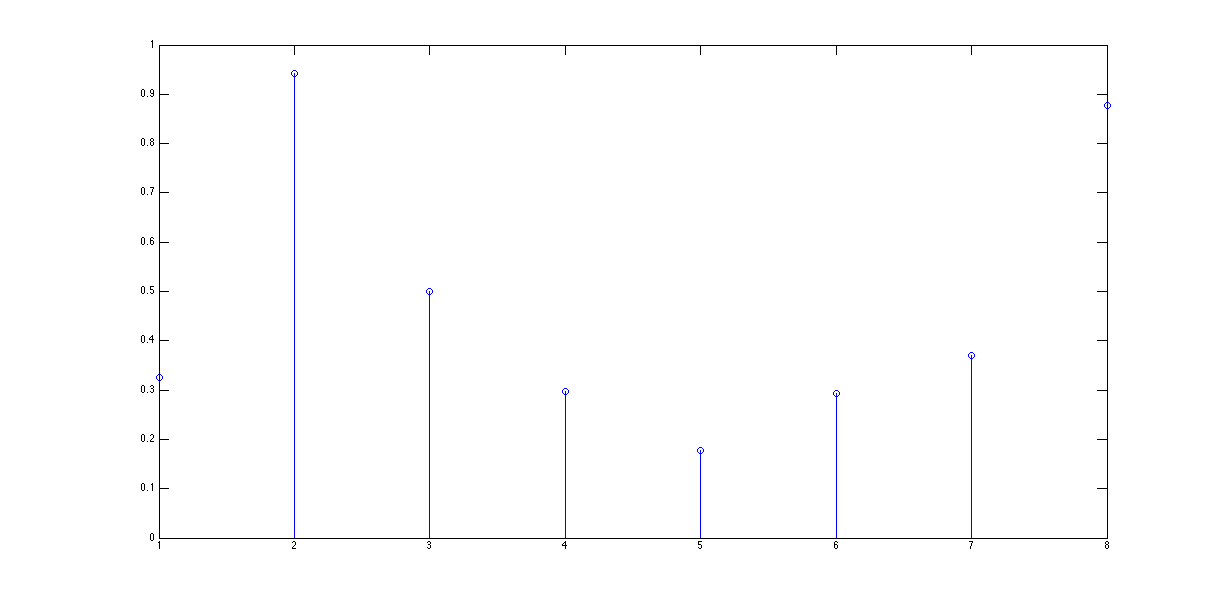
\includegraphics[width=\textwidth]{goertzelVis.png}
  \caption{Absolute Beträge der Ergebnisse des Goertzel-Algortihmus}
  \label{fig:Goertzel}
\end{figure}
In \autoref{fig:Goertzel} ist zu sehen, dass jeweils der 2. und der 8. Wert im Vergleich zu den Anderen relativ hoch ist. Da wir aber nur einen hohen Wert erwarteten gehen wir (in Absprache mit Herrn Purat) davon aus, dass der Goertzel-Algorithmus nicht wie erwartet funktioniert.
Dahingegen ist in \autoref{fig:FFT} zu sehen, dass es ein ganz klares Maximum gibt.
\begin{figure}[H]
	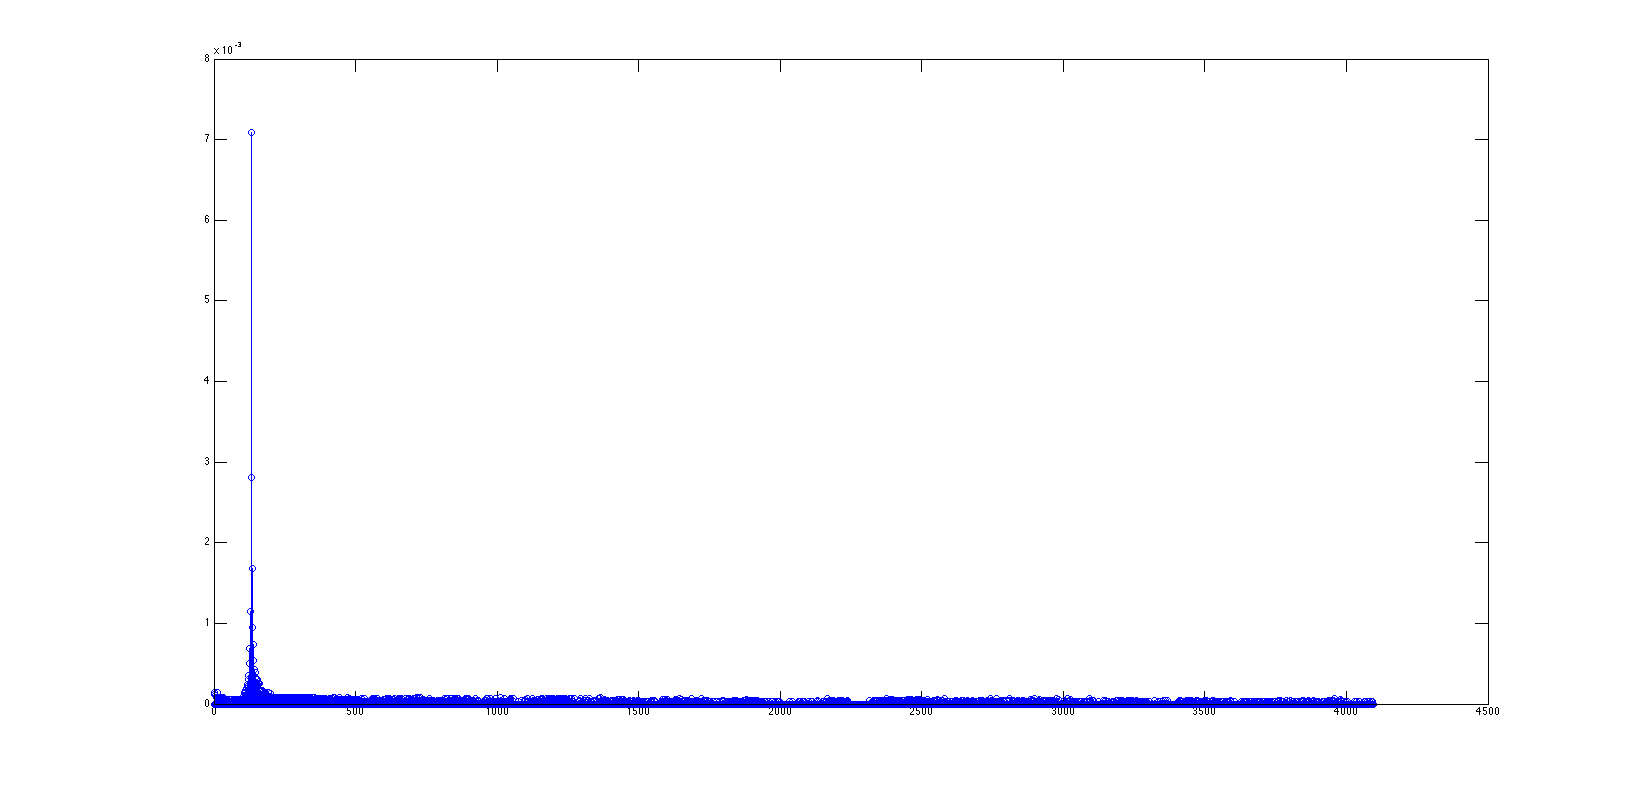
\includegraphics[width=\textwidth]{FFTVis.png}
  \caption{Absolute Beträge der Ergebnisse des FFT-Algortihmus}
  \label{fig:FFT}
\end{figure}
Im Weiteren soll der Rechenaufwand beider Implementierungen verglichen werden.
\begin{center}
	\begin{tabular}{l|c|c}
	 & Goertzel-Algorthmus & FFT-Algorithmus \\ \hline
	 Rechenaufwand in Maschinenzyklen & 1524110 & 3727089
	\end{tabular}
\end{center} 
Die Tabelle zeigt, dass der Goertzel-Algorithmus deutlich schneller ist. In unserem Beispiel um einen Faktor von 2,4. Dies liegt daran, dass der Goertzel Algorithmus nur noch die Spektralwerte an genau den Stellen der DTMF Frequenzen errechnet und nicht wie die FFT über einen gesamten Block von 4096 Werten.




\clearpage\newpage
\listoffigures

\printnoidxglossary[type=\acronymtype,title=Abkürzungsverzeichnis]

\end{document}